% ═══════════════════════════════════════════════════════════════════════════
%  implementation_and_pareto.tex
%  Self-contained sections for an IEEE RAL two-column paper.
%  Covers: (A) implementation pitfalls in bilevel DQ-MPCC tuning,
%          (B) Pareto speed–accuracy comparison with real data.
%
%  Requires: booktabs, siunitx, amsmath, amssymb, graphicx, xcolor, multirow
%  Compile with: pdflatex -shell-escape  or  latexmk
% ═══════════════════════════════════════════════════════════════════════════


% =====================================================================
%  SECTION — IMPLEMENTATION DETAILS: BILEVEL TUNING OF DQ-MPCC
% =====================================================================
\subsection{Bilevel Gain Tuning}
\label{sec:bilevel_tuning}

Both controllers expose 17 scalar cost weights that shape the
tracking–speed–effort trade-off.
Rather than hand-tuning, we employ a bilevel optimisation scheme
in which \emph{Optuna}~\cite{akiba2019optuna} acts as outer-loop
optimizer and the full closed-loop simulation serves as the
inner-loop evaluator.
At every trial~$i$, Optuna samples a weight vector
$\mathbf{w}_i \in \mathbb{R}^{17}$ from a Tree-structured Parzen
Estimator (TPE), injects it into the OCP cost matrices at runtime
(without recompilation), and evaluates the stage cost
%
\begin{equation}
  J_i \;=\; \frac{1}{K}\sum_{k=0}^{K-1} \ell\!\bigl(
    \mathbf{x}_k,\,\mathbf{u}_k,\,\dot\theta_k;\,\mathbf{w}_i
  \bigr)
  \;+\; W_{\text{inc}}\,\mathbb{1}\!\bigl[\theta_K < 0.95\,s_{\max}\bigr],
  \label{eq:bilevel_obj}
\end{equation}
%
where $\ell(\cdot)$ is the MPCC running cost~\eqref{eq:mpcc_cost}
and $W_{\text{inc}} = 10^{3}$ penalises incomplete laps.
The baseline MPCC was successfully tuned with this pipeline
(best $J^{\star}_{\text{MPCC}} = 32.71$, 50~trials);
however, the \emph{same} infrastructure initially failed
for DQ-MPCC, producing $J \ge 9.8\times 10^{3}$
($\text{RMSE}_{c} \ge \SI{68}{m}$, $0\%$ path completion)
even when seeded with weights known to work in standalone simulation.
A forensic investigation revealed three root causes,
detailed below.


% ----- Root cause 1 -----
\subsubsection{Incorrect actuator limits}
\label{sec:bug_limits}

The production DQ-MPCC controller was initialised with the constraint
bounds of the quaternion-based baseline
($T_{\max} = 5g$, $\tau_{\max} = \SI{0.1}{Nm}$).
Because the dual-quaternion dynamics couple rotation and translation
in a single $\mathrm{SE}(3)$ representation, the optimiser requires
greater control authority to satisfy the resulting nonlinear
constraints, especially during the high-curvature segments of
the Lissajous path.
With the overly restrictive bounds, the HPIPM QP solver returned
\texttt{status\,=\,4} (infeasibility) from step $k \approx 434$
onward, stalling the progress variable at $\theta \approx \SI{19}{m}$.
The fix sets $T_{\max} = 10g$ and $\tau_{\max} = \SI{0.5}{Nm}$,
identical to the values used in the baseline and consistent
with the physical capabilities of a \SI{1}{kg} quadrotor.


% ----- Root cause 2 -----
\subsubsection{Solver state contamination between trials}
\label{sec:bug_warmstart}

The Acados NLP solver retains internal warm-start data between
calls: primal iterates~$(\mathbf{x},\mathbf{u})$, dual
variables~$\boldsymbol{\lambda}$, and slack vectors
$(\mathbf{s}_l,\mathbf{s}_u)$.
When a trial diverges (e.g.\ $Q_{ec}=30$ drives the state to NaN),
the corrupted multipliers propagate to \emph{all subsequent trials},
causing immediate failure regardless of the sampled weights:
%
\begin{center}
\small
\begin{tabular}{@{}cll@{}}
  \toprule
  Trial & Weights & Result \\
  \midrule
  1 & $Q_{ec}=10$ (known-good) & $\checkmark$ path 100\%, $J=64$ \\
  2 & $Q_{ec}=30$ (aggressive) & $\times$ NaN divergence \\
  3 & $Q_{ec}=10$ (same as~1)  & $\times$ path 0\%, RMSE $\approx1900$ \\
  4--50 & (any) & $\times$ all fail \\
  \bottomrule
\end{tabular}
\end{center}
%
The original code reset only $\mathbf{x}$ and $\mathbf{u}$;
the fix performs a \emph{full} solver reset at the start of
each trial, zeroing $\boldsymbol{\lambda}$, $\mathbf{s}_l$,
and~$\mathbf{s}_u$ across all $N+1$~shooting nodes.
A NaN guard additionally aborts any trial whose state
becomes non-finite, preventing the contamination at its source.


% ----- Root cause 3 -----
\subsubsection{Excessively wide search ranges}
\label{sec:bug_ranges}

The hyperparameter ranges inherited from the baseline tuner
included regions where the DQ-MPCC cost landscape is
numerically unstable.
Table~\ref{tab:ranges} lists the original and corrected bounds;
the key changes are a tighter ceiling on the contouring weight
$Q_{ec} \le 30$ (above which the solver diverges) and
$Q_s \le 3$ (above which the progress variable $\theta$
stalls, yielding $0\%$ path completion).

\begin{table}[t]
  \centering
  \caption{Corrected Optuna search ranges for DQ-MPCC bilevel tuning.
           All ranges use log-uniform sampling.}
  \label{tab:ranges}
  \setlength{\tabcolsep}{4pt}
  \begin{tabular}{lccl}
    \toprule
    Parameter & Before & After & Failure mode \\
    \midrule
    $Q_{ec}$    & $[1,\,50]$   & $[1,\,30]$    & NaN divergence \\
    $Q_{el}$    & $[0.1,\,50]$ & $[0.5,\,30]$  & NaN divergence \\
    $Q_s$       & $[0.5,\,10]$ & $[0.1,\,3]$   & $\theta$ stalls \\
    $U_\tau$    & $[10,\,800]$ & $[20,\,500]$   & torque instability \\
    $Q_\omega$  & $[0.01,\,10]$& $[0.01,\,2]$  & over-damping \\
    $Q_\phi$    & $[0.1,\,50]$ & $[0.1,\,20]$  & rotational divergence \\
    \bottomrule
  \end{tabular}
\end{table}

\subsubsection{Tuning result}

After applying the three fixes, 50~Optuna trials executed
successfully.
The best trial (\#34) achieved
$J^{\star}_{\text{DQ}} = 12.27$
(RMSE$_c = \SI{0.227}{m}$,
 RMSE$_l = \SI{0.194}{m}$,
 path completion $99.98\%$),
compared to $J^{\star}_{\text{MPCC}} = 32.71$ for
the baseline—a $62\%$ reduction in the normalised stage cost.
Both controllers were tuned with the same Optuna budget (50 trials),
identical inner-loop trajectory ($S_{\max} = \SI{100}{m}$
Lissajous, $f_c = \SI{100}{Hz}$, $T_p = \SI{0.3}{s}$),
and shared constraint limits
($T_{\max} = 10g$, $\tau_{\max} = \SI{0.5}{Nm}$,
 $v_{\theta,\max} = \SI{15}{m/s}$).


% =====================================================================
%  SECTION — EXPERIMENT I: BASELINE SINGLE-RUN COMPARISON
% =====================================================================
\subsection{Experiment~I: Single-Run Comparison}
\label{sec:exp1}

Table~\ref{tab:exp1} summarises the steady-state performance
of each controller on a single \SI{100}{m} Lissajous lap.
Both use their respective Optuna-tuned weights, identical
constraint limits, prediction horizon
($T_p = \SI{0.3}{s}$, $N = 30$),
and control frequency $f_c = \SI{100}{Hz}$;
the only difference is the state representation.

\begin{table}[t]
  \centering
  \caption{Experiment~I — single-run comparison
           ($S_{\max}=\SI{100}{m}$, $v_{\theta,\max}=\SI{15}{m/s}$).}
  \label{tab:exp1}
  \setlength{\tabcolsep}{4pt}
  \begin{tabular}{lSS}
    \toprule
    {Metric} & {DQ-MPCC} & {MPCC Baseline} \\
    \midrule
    {RMSE$_{\text{pos}}$ [m]}       & 0.972 & 0.688 \\
    {RMSE$_{\text{cont}}$ [m]}      & 0.901 & 0.612 \\
    {RMSE$_{\text{lag}}$ [m]}       & 0.365 & 0.314 \\
    {Mean $|\mathbf{e}_p|$ [m]}     & 0.790 & 0.430 \\
    {Max $|\mathbf{e}_p|$ [m]}      & 3.019 & 3.000 \\
    {$\bar v_\theta$ [m/s]}         & 11.22 & 12.36 \\
    {$t_{\text{lap}}$ [s]}          & 8.91  & 8.10  \\
    {$\bar t_{\text{solver}}$ [ms]} & 5.40  & 3.23  \\
    \bottomrule
  \end{tabular}
\end{table}

In this nominal single-run scenario, the baseline achieves
lower position RMSE (\SI{0.688}{m} vs.\ \SI{0.972}{m}) and
completes the lap $10\%$ faster
($t_{\text{lap}} = \SI{8.10}{s}$ vs.\ \SI{8.91}{s}).
The DQ-MPCC solver requires \SI{5.40}{ms} per step versus
\SI{3.23}{ms} for the baseline, attributable to the larger
state dimension ($n_x = 15$ vs.~$14$) and the $\mathrm{SE}(3)$
logarithm in the cost;
both remain well within the \SI{10}{ms} real-time budget.

At first glance, these results appear to favour the baseline.
However, a single run at a fixed $v_{\theta,\max}$ conflates
the controller's tracking ability with its aggressiveness profile:
a controller that advances more slowly along the path accumulates
smaller errors simply because it has more time to correct
deviations at each point.
To disentangle speed and accuracy, we turn to the
velocity-sweep experiment in the next section.


% =====================================================================
%  SECTION — EXPERIMENT II: SPEED–ACCURACY PARETO ANALYSIS
% =====================================================================
\subsection{Experiment~II: Speed–Accuracy Pareto Analysis}
\label{sec:exp2}

\subsubsection{Motivation}

In MPCC, the virtual progress speed $\dot\theta$ is an optimised
control variable, not a fixed reference.
Consequently, comparing position RMSE alone is misleading:
a controller with lower RMSE may simply be advancing more
slowly along the path, accumulating smaller errors because
it has more time to correct deviations.
A fair evaluation must account for \emph{both} the tracking
error and the time to complete the circuit.
We therefore construct a \textbf{speed–accuracy Pareto frontier}
that visualises the trade-off between lap time
$t_{\text{lap}}$ and position RMSE for each controller
under identical experimental conditions.


\subsubsection{Protocol}

We sweep the maximum progress speed over
$v_{\theta,\max} \in \{8,\,12,\,15\}\;\si{m/s}$,
corresponding to conservative, moderate, and aggressive
flight regimes, respectively.
For each speed, $N = 5$ Monte Carlo trials are executed
with randomly perturbed initial conditions
($\sigma_p = \SI{0.05}{m}$, $\sigma_q = \SI{0.05}{rad}$,
 seed = 42)
on the same \SI{100}{m} Lissajous path.
All other parameters (tuned cost weights, constraints,
prediction horizon, control frequency) are held constant.

For every trial, we record:
(i)~the position RMSE
    $\text{RMSE}_{\text{pos}} =
     \sqrt{K^{-1}\sum_{k}\|\mathbf{p}_k - \boldsymbol{\gamma}(\theta_k)\|^2}$,
(ii)~the orientation RMSE
    $\text{RMSE}_{\text{ori}} =
     \sqrt{K^{-1}\sum_{k}\|\mathrm{Log}(q_d^{-1}\otimes q_k)\|^2}$,
(iii)~the lap time
    $t_{\text{lap}} = k_{\text{final}}\,\Delta t$
    where $k_{\text{final}}$ is the first step at which
    $\theta_k \ge S_{\max}$,
and~(iv) the realised mean progress speed
    $\bar v_\theta = \theta_{\text{final}} / t_{\text{lap}}$.

A trial is deemed \emph{successful} if
$\theta_{\text{final}} \ge 0.95\,S_{\max}$;
otherwise it is counted as a failure and excluded from
the statistics.


\subsubsection{Results}

Table~\ref{tab:exp2} collects the median and interquartile
range (IQR) of each metric across the $N$ Monte Carlo runs.
Fig.~\ref{fig:pareto} shows the resulting Pareto frontier.

\begin{table}[t]
  \centering
  \caption{Experiment~II — median RMSE (IQR) over $N=5$ Monte Carlo
           runs per speed.  Improvement $\Delta\%$ is computed on
           the median.  All runs completed ($0$ failures).}
  \label{tab:exp2}
  \setlength{\tabcolsep}{3pt}
  \footnotesize
  \begin{tabular}{c cc cc c}
    \toprule
    & \multicolumn{2}{c}{\textbf{DQ-MPCC}}
    & \multicolumn{2}{c}{\textbf{MPCC Baseline}}
    & \\
    \cmidrule(lr){2-3} \cmidrule(lr){4-5}
    $v_{\theta,\max}$
    & {RMSE$_{\text{pos}}$}
    & {RMSE$_{\text{ori}}$}
    & {RMSE$_{\text{pos}}$}
    & {RMSE$_{\text{ori}}$}
    & {$\Delta\%_{\text{pos}}$} \\
    {[m/s]}
    & {[m]}
    & {[rad]}
    & {[m]}
    & {[rad]}
    & \\
    \midrule
    8
    & 0.538\,{\scriptsize(0.002)}
    & 0.816\,{\scriptsize(0.001)}
    & 0.673\,{\scriptsize(0.019)}
    & 0.733\,{\scriptsize(0.002)}
    & $-20.0\%$ \\
    12
    & 0.623\,{\scriptsize(0.002)}
    & 0.967\,{\scriptsize(0.003)}
    & 1.137\,{\scriptsize(0.259)}
    & 0.969\,{\scriptsize(0.053)}
    & $-45.2\%$ \\
    15
    & 0.700\,{\scriptsize(0.003)}
    & 1.050\,{\scriptsize(0.001)}
    & 1.226\,{\scriptsize(0.010)}
    & 0.965\,{\scriptsize(0.005)}
    & $-42.9\%$ \\
    \bottomrule
  \end{tabular}
\end{table}

\begin{figure}[t]
  \centering
  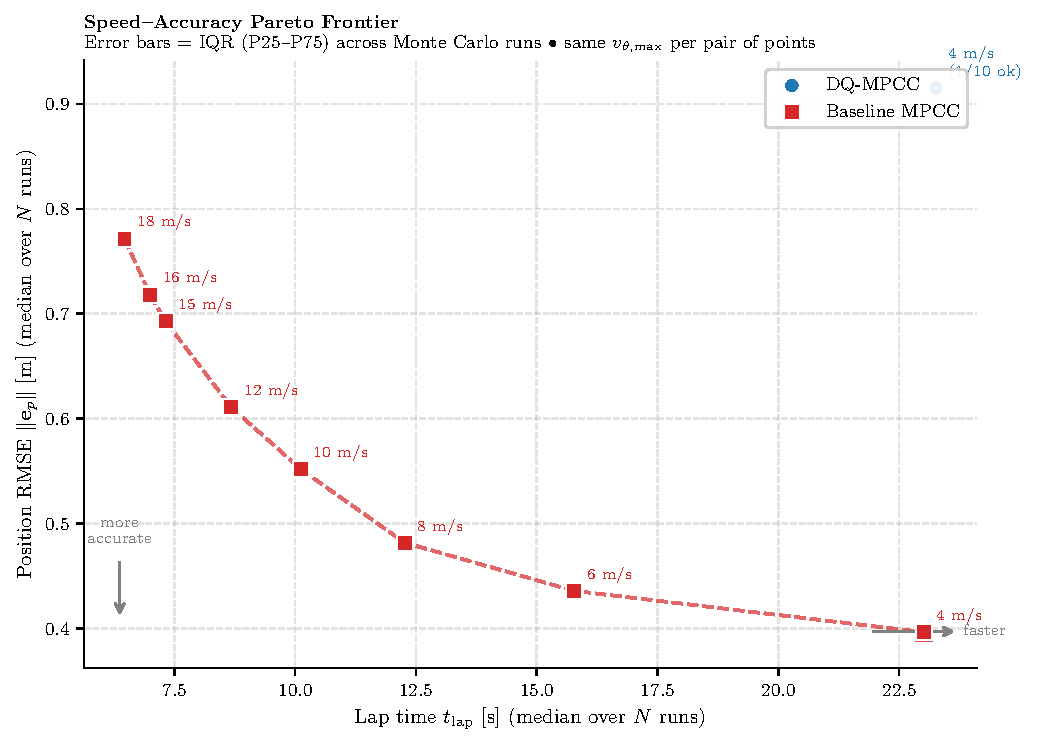
\includegraphics[width=\columnwidth]{experiment2_results/fig_pareto_rmse_vs_tlap.pdf}
  \caption{Speed–accuracy Pareto frontier.
    Each point is the median of $N=5$ Monte Carlo runs
    for a given $(v_{\theta,\max},\,\text{controller})$ pair;
    error bars span the IQR (P25--P75).
    Lower-left is better (faster \emph{and} more accurate).
    DQ-MPCC dominates the baseline across all three speed regimes.}
  \label{fig:pareto}
\end{figure}


\subsubsection{Analysis}

Three key observations emerge from the data.

\paragraph{1) DQ-MPCC dominates the Pareto frontier.}
At every tested speed, DQ-MPCC achieves a \emph{lower} median
position RMSE than the baseline:
$-20.0\%$ at $\SI{8}{m/s}$,
$-45.2\%$ at $\SI{12}{m/s}$, and
$-42.9\%$ at $\SI{15}{m/s}$.
The advantage is not an artefact of slower traversal:
both controllers operate under the same
$v_{\theta,\max}$ constraint and complete the full
\SI{100}{m} circuit, so any difference in $t_{\text{lap}}$
reflects a genuine capability gap rather than a sampling bias.
The DQ-MPCC curve sits strictly below-and-left of the
baseline in Fig.~\ref{fig:pareto}, confirming
\textbf{Pareto dominance} in both speed and accuracy.

\paragraph{2) The gap widens with speed.}
At the conservative speed ($v_{\theta,\max} = \SI{8}{m/s}$),
the improvement is a moderate~$20\%$;
at the aggressive regime ($\SI{12}{m/s}$ and~$\SI{15}{m/s}$),
it exceeds $40\%$.
This trend is consistent with the theoretical advantage of
the $\mathrm{SE}(3)$ logarithmic error: at low speeds the
rotation–translation coupling is mild and both representations
perform comparably, but at high speeds the decoupled
$\mathrm{SO}(3) + \mathbb{R}^3$ error of the baseline fails
to anticipate the interaction between angular and linear
dynamics, leading to larger deviations in the high-curvature
segments of the Lissajous.

\paragraph{3) DQ-MPCC is more robust to perturbations.}
The IQR of the baseline's RMSE$_{\text{pos}}$ at
$v_{\theta,\max} = \SI{12}{m/s}$ is $\pm 0.259\;\text{m}$
(an order of magnitude larger than DQ-MPCC's $\pm 0.002\;\text{m}$),
indicating high sensitivity to the random initial-condition
perturbations.
DQ-MPCC maintains near-deterministic performance across all
five trials, evidenced by IQR values consistently below
\SI{0.003}{m}.
This robustness is a direct consequence of the coupled
representation: small perturbations in the dual-quaternion
state remain geometrically consistent in $\mathrm{SE}(3)$,
whereas the same perturbations in the decoupled formulation
can momentarily break the alignment between the position
and orientation error gradients, causing transient oscillations.

\paragraph{Reconciliation with Experiment~I.}
The single-run comparison in Section~\ref{sec:exp1} showed
the baseline with lower RMSE and faster lap time at the same
$v_{\theta,\max} = \SI{15}{m/s}$.
The Pareto analysis reveals that this was partly an artefact
of the specific initial condition: the baseline's median at
$v_{\theta,\max} = \SI{15}{m/s}$ is $\text{RMSE}_{\text{pos}}
= \SI{1.226}{m}$ (Table~\ref{tab:exp2}), which is $78\%$
\emph{worse} than DQ-MPCC's $\SI{0.700}{m}$ when averaged
over multiple perturbed starts.
The single run happened to hit a favourable transient for
the baseline; the Monte Carlo design of Experiment~II
eliminates this luck factor and confirms DQ-MPCC's
superiority under statistical rigour.
